% !TEX root = ../../seminar.tex

\section{Research Process - \checklist}
\label{sec:research process}

\begin{minipage}{\linewidth}
\begin{wrapfigure}{R}{0.3\textwidth}
	\centering
	\vspace{-1.0cm}
	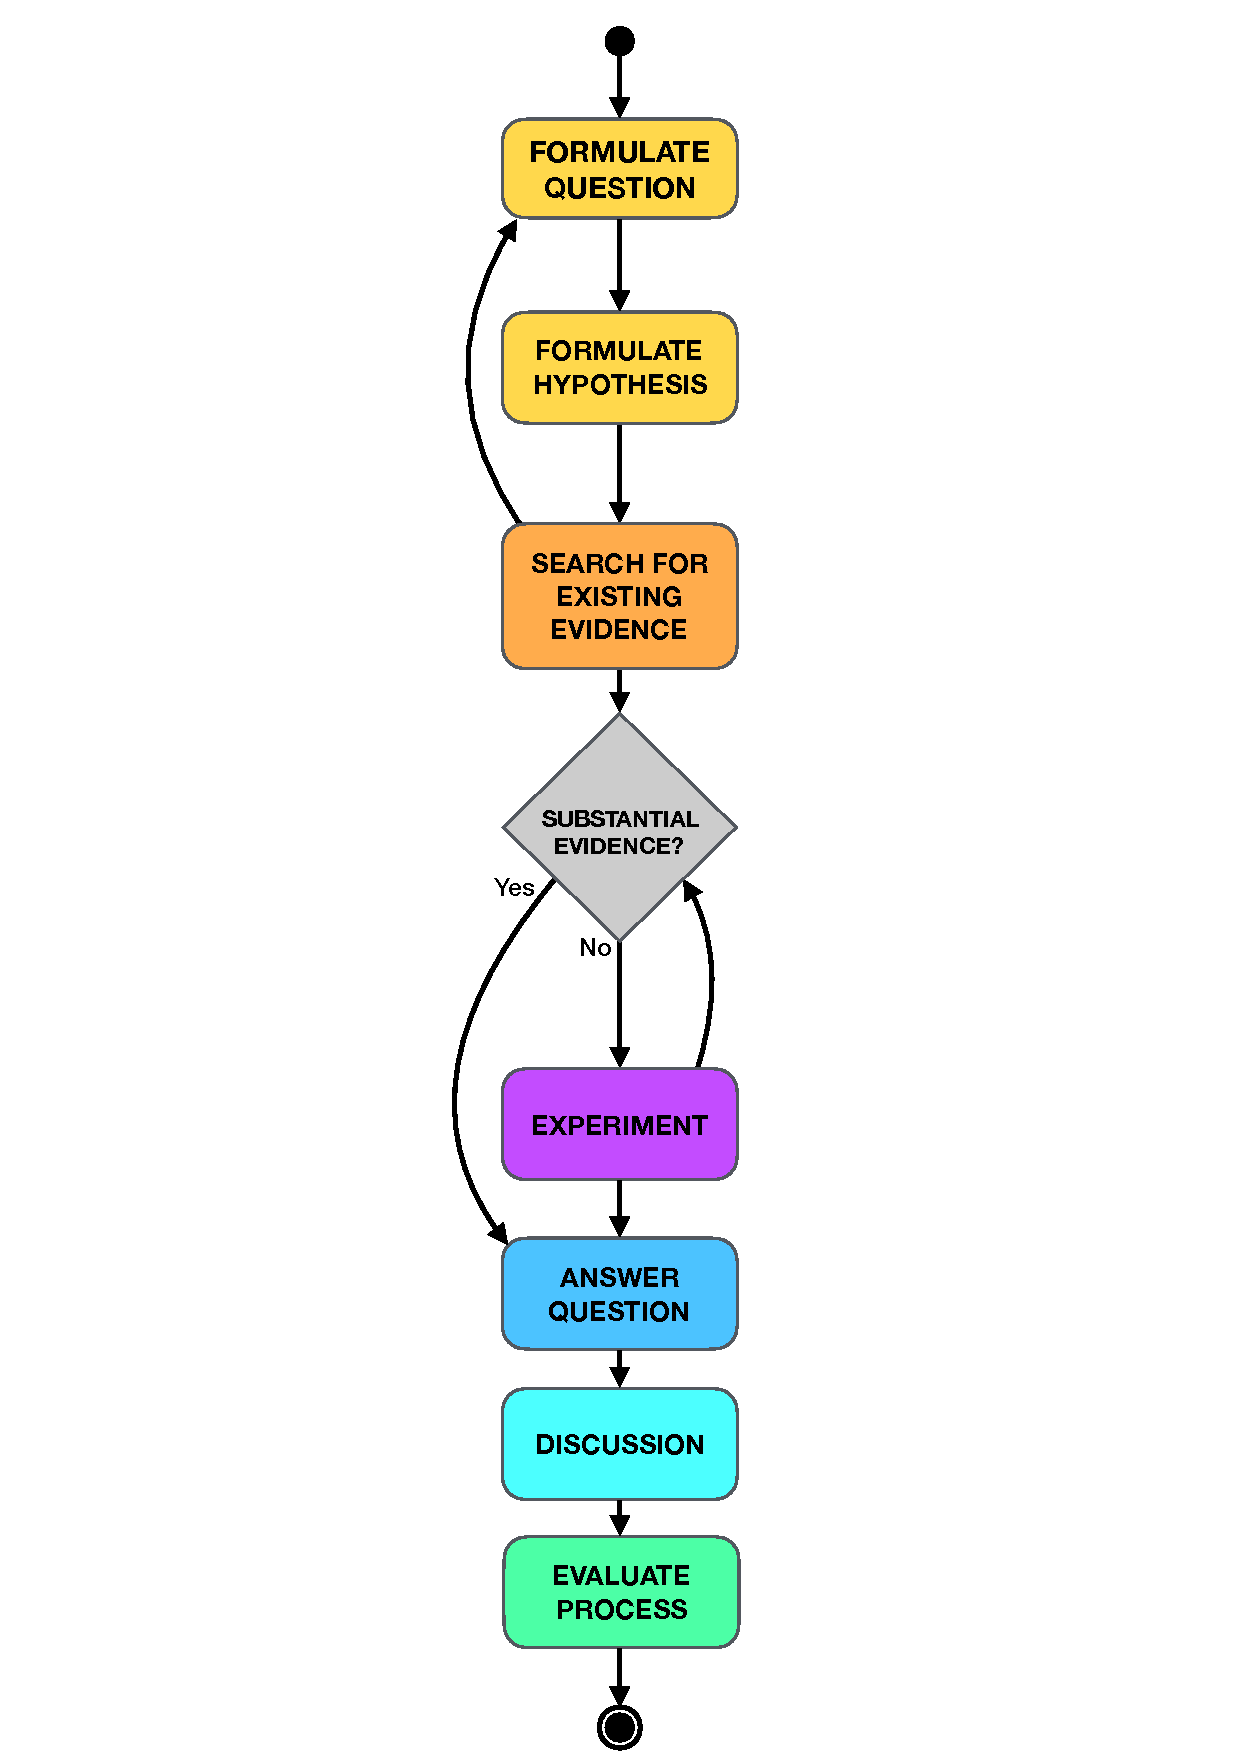
\includegraphics[trim={3cm 0 3cm 0}, height=14.55cm]{figures/workflow_graph.pdf}
	\caption{Workflow Graph}
	\label{fig:workflow_graph}
\end{wrapfigure}



In this section, a document called \emph{\checklist} is introduced. It is supposed to guide students through scientific working with EBSE in mind.

Rainer \etal found, that \q{[s]tudents varied in their use of the EBSE checklist} \cite{Rainer2006} (see issue \ref{itm:issue5} in table \ref{table:issuesEBSE}). Therefore, an important design criteria for \checklist is ease of use through clear and simple instructions. Especially tailored for students with little knowledge about scientific working in general.

The process of \checklist contains eight steps:
\begin{enumerate}
\item Formulate question
\item Formulate hypothesis
\item Search for existing evidence
\item Substantial evidence
\item Experiment
\item Answer question
\item Discussion
\item Evaluate process
\end{enumerate}


The whole graph can be seen in figure \ref{fig:workflow_graph}. The actual document can be found in appendix \ref{appendix:checklist}.\\
On the left of the document, a flow chart of the proposed process is depicted. For computer science students this should be a fast way to navigate through and orient themselves in the process. To further assist navigation visually, each process step has been assigned a unique color. This color schemes reoccurs in the tools section of the document as well as in \briefingform.

On the right additional information is given. Each process step in \checklist contains a short description, some guidelines, and acceptance criteria. The guidelines contain methods and tools on how to process the current step. The acceptance criteria give students orientation on when a step is completed.
\end{minipage}









